\documentclass[12pt]{article}

\usepackage{geometry}
\geometry{a4paper}

\usepackage{graphicx}
\usepackage{amssymb}
\usepackage{physics}
\usepackage{amsmath}
\usepackage{lipsum}

\usepackage{cite} %Uses proper indexing when citing multiple papers
\usepackage{authblk} %Shows all authors with e-mail addresses and affiliations properly on the page

%%%%%%%%%%%%%%%%%%%%%%%%%%%%%%% INFO %%%%%%%%%%%%%%%%%%%%%%%%%%%%%%%%%%%%%%%%%
\title{Extensive Study of the Wobbling Properties in $^{163}$Lu Based on the Parity Concept} 

\author[1,2]{Robert Poenaru \thanks{E-mail: robert.poenaru@drd.unibuc.ro}}
\author[2,3]{Apolodor Aristotel Raduta \thanks{E-mail: raduta@nipne.ro}}

\affil[1]{Doctoral School of Physics, University of Bucharest, Romania}
\affil[2]{\textit{Horia Hulubei} National Institute for Physics and Nuclear Engineering, M\u{a}gurele-Bucharest, Romania}
\affil[3]{Academy of Romanian Scientists, Bucharest, Romania}
%%%%%%%%%%%%%%%%%%%%%%%%%%%%%%% INFO %%%%%%%%%%%%%%%%%%%%%%%%%%%%%%%%%%%%%%%%%

\date{\today}

\begin{document}

\bibliographystyle{unsrt}

\maketitle

%%%%%%%%%%%%%%%%%%%%%%%%%%%%%%% TEXT %%%%%%%%%%%%%%%%%%%%%%%%%%%%%%%%%%%%%%%%%
\begin{abstract}
A new interpretation on the wobbling structure in $^{163}$Lu is developed, based on the concept of parity symmetry. It is known that four wobbling bands are experimentally observed in this isotope, where three of them are considered as wobbling phonon excitations (namely $TSD_2$, $TSD_3$, and $TSD_4$) and the yrast band for the ground state (that is TSD1). In the present work, the trial function that is used for obtaining the wobbling spectrum is analyzed in terms of its behavior under the rotation operation. Indeed, due to a specific symmetry to rotations with $\pi$ around the 2-axis of the triaxial system, the parity becomes a good quantum number. As such, the trial function admits solutions with negative parity, which belong to the rotational states in $TSD_4$. A unified description of all the triaxial super-deformed bands in $^{163}$Lu is achieved with the new formalism.
\end{abstract}

\section{Introduction}
Wobbling motion in nuclei was extensively studied in the recent years, and the scientific community finally shed some light on this elusive phenomenon. This kind of collective motion was firstly predicted by Bohr and Mottelson, more than 50 years ago \cite{bohr1998nuclear}.

\section{Theoretical Background}

In a previous work, a complete description of the triaxial characteristics of the Lu isotopes was given, where results for the wobbling energies and transition probabilities were presented \cite{raduta2018wobbling}.

A new interpretation on the wobbling motion, but based on the quasiparticle plus triaxial rotor model was given recently by Chen et. al. \cite{chen2020interpretation}.

\begin{align}
    \ket{\Psi}=1
    \label{wavefunction}
\end{align}

The equation \ref{wavefunction} is good. This equation is studied in detail by the same team in \cite{raduta2018wobbling} and also \cite{raduta2020new}.
Nuclear wobbling motion was first predicted theoretically for even-even nuclei \cite{bohr1998nuclear}. The references \cite{bohr1998nuclear,raduta2018wobbling,chen2020interpretation,raduta2020new} contain valid information.

\section{Energy function $\mathcal{H}$}

It is worth analyzing the energy function in terms of its numerical evolution with the change in spin. As such, evaluation in critical point which behaves as a minimum of $\mathcal{H}$ (considering the MOI ordering that was obtained throughout the fitting procedure) was studied, with the numerical evolution shown in Figure \ref{energy_function_min_point}.

\begin{figure}
    \centering
    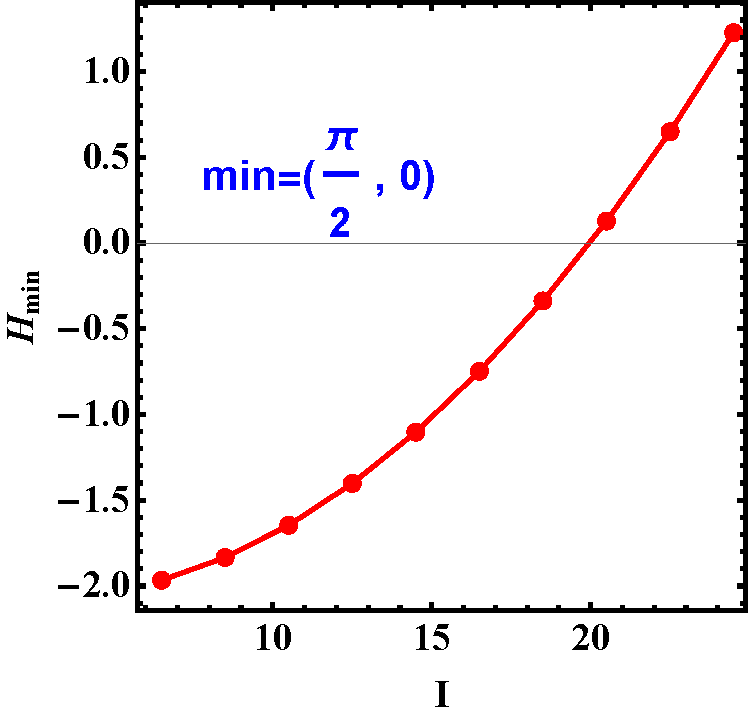
\includegraphics[scale=0.5]{dev-draft/figs/EnergyFunction_minPointEvolution_low.pdf}
    \caption{The evolution of the energy function in a critical point, with respect to the total angular momentum of the rotor.}
    \label{energy_function_min_point}
\end{figure}

%%%%%%%%%%%%%%%%%%%%%%%%%%%%%%% TEXT  %%%%%%%%%%%%%%%%%%%%%%%%%%%%%%%%%%%%%%%%%

\bibliography{references}

\end{document}  